\section{Verwendete Hardware}
\label{sec:verwendeteHardware}
Als Zielplattform für diese Arbeit dient ein Raspberry Pi 4B. Der Raspberry Pi 4B
verfügt dabei unter anderem über die folgenden technischen Spezifikationen: \cite{RasberryPiSpecs}
\begin{itemize}
    \item 1,5 GHz ARM Cortex-A72 Quad-Core-CPU
    \item 4 GB LPDDR4 SDRAM
    \item Gigabit LAN RJ45 (bis zu 1000 Mbit)
    \item Bluetooth 5.0
    \item 2x USB 2.0 / 2x USB 3.0
    \item 2x microHDMI
    \item 5V/3A @ USB Typ-C
    \item 40 GPIO Pins
    \item Mikro SD-Karten Slot
\end{itemize}
Der Raspberry Pi 4B wird mit dem \emph{Raspbian Buster with desktop} auf der SD-Karte betrieben.
\newline
Um noch mehr Funktionalität aufbringen zu können, wurde auf dem Raspberry Pi ein
\emph{RPI SENSE HAT Shield} aufgesteckt. Mithilfe des \emph{RPI SENSE HAT Shield} können dann
unter anderem Daten, wie zum Beispiel die momentane Temperatur, oder auch die momentane
Luftfeuchtigkeit gewonnen werden. Zudem ist auf dem Raspberry Pi noch eine 8x8 LED-Matrix enthalten
und ein Joystick mit 5 Knöpfen, die eingelesen werden können.
\begin{figure}[h]
    \centering
    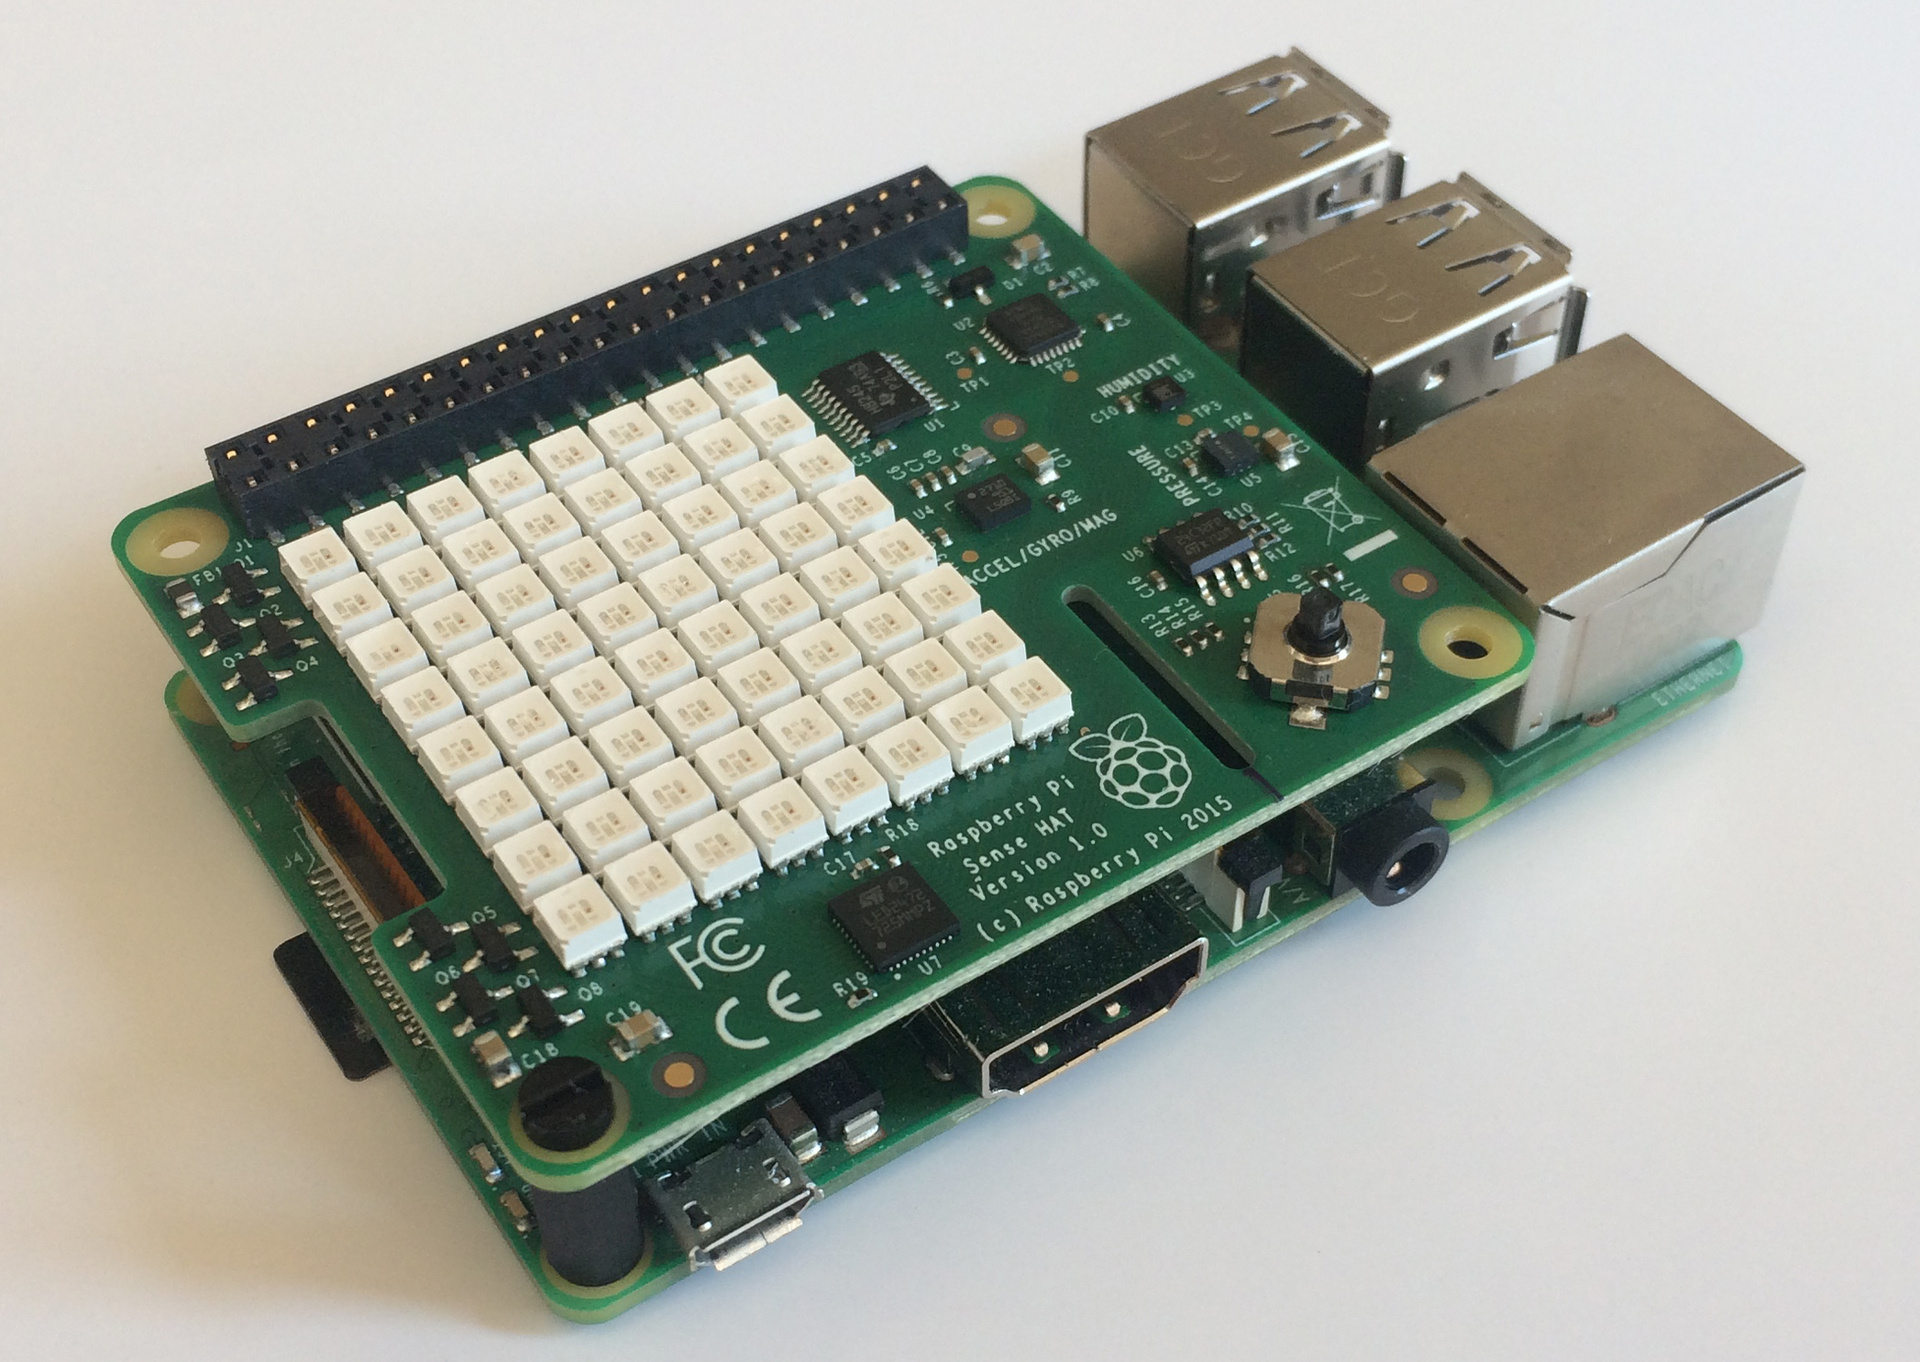
\includegraphics[width=0.5\textwidth, center]{Einleitung/pi-sense}
    \caption[Raspberry Pi 4 B]{Verwendeter Raspberry Pi}
    \label{img:piSense}
\end{figure}

